% Options for packages loaded elsewhere
\PassOptionsToPackage{unicode}{hyperref}
\PassOptionsToPackage{hyphens}{url}
%
\documentclass[
  ignorenonframetext,
]{beamer}
\usepackage{pgfpages}
\setbeamertemplate{caption}[numbered]
\setbeamertemplate{caption label separator}{: }
\setbeamercolor{caption name}{fg=normal text.fg}
\beamertemplatenavigationsymbolshorizontal
% Prevent slide breaks in the middle of a paragraph
\widowpenalties 1 10000
\raggedbottom
\setbeamertemplate{part page}{
  \centering
  \begin{beamercolorbox}[sep=16pt,center]{part title}
    \usebeamerfont{part title}\insertpart\par
  \end{beamercolorbox}
}
\setbeamertemplate{section page}{
  \centering
  \begin{beamercolorbox}[sep=12pt,center]{part title}
    \usebeamerfont{section title}\insertsection\par
  \end{beamercolorbox}
}
\setbeamertemplate{subsection page}{
  \centering
  \begin{beamercolorbox}[sep=8pt,center]{part title}
    \usebeamerfont{subsection title}\insertsubsection\par
  \end{beamercolorbox}
}
\AtBeginPart{
  \frame{\partpage}
}
\AtBeginSection{
  \ifbibliography
  \else
    \frame{\sectionpage}
  \fi
}
\AtBeginSubsection{
  \frame{\subsectionpage}
}

\usepackage{amsmath,amssymb}
\usepackage{iftex}
\ifPDFTeX
  \usepackage[T1]{fontenc}
  \usepackage[utf8]{inputenc}
  \usepackage{textcomp} % provide euro and other symbols
\else % if luatex or xetex
  \usepackage{unicode-math}
  \defaultfontfeatures{Scale=MatchLowercase}
  \defaultfontfeatures[\rmfamily]{Ligatures=TeX,Scale=1}
\fi
\usepackage{lmodern}
\usetheme[]{AnnArbor}
\usecolortheme{lily}
\ifPDFTeX\else  
    % xetex/luatex font selection
\fi
% Use upquote if available, for straight quotes in verbatim environments
\IfFileExists{upquote.sty}{\usepackage{upquote}}{}
\IfFileExists{microtype.sty}{% use microtype if available
  \usepackage[]{microtype}
  \UseMicrotypeSet[protrusion]{basicmath} % disable protrusion for tt fonts
}{}
\makeatletter
\@ifundefined{KOMAClassName}{% if non-KOMA class
  \IfFileExists{parskip.sty}{%
    \usepackage{parskip}
  }{% else
    \setlength{\parindent}{0pt}
    \setlength{\parskip}{6pt plus 2pt minus 1pt}}
}{% if KOMA class
  \KOMAoptions{parskip=half}}
\makeatother
\usepackage{xcolor}
\newif\ifbibliography
\setlength{\emergencystretch}{3em} % prevent overfull lines
\setcounter{secnumdepth}{-\maxdimen} % remove section numbering


\providecommand{\tightlist}{%
  \setlength{\itemsep}{0pt}\setlength{\parskip}{0pt}}\usepackage{longtable,booktabs,array}
\usepackage{calc} % for calculating minipage widths
\usepackage{caption}
% Make caption package work with longtable
\makeatletter
\def\fnum@table{\tablename~\thetable}
\makeatother
\usepackage{graphicx}
\makeatletter
\def\maxwidth{\ifdim\Gin@nat@width>\linewidth\linewidth\else\Gin@nat@width\fi}
\def\maxheight{\ifdim\Gin@nat@height>\textheight\textheight\else\Gin@nat@height\fi}
\makeatother
% Scale images if necessary, so that they will not overflow the page
% margins by default, and it is still possible to overwrite the defaults
% using explicit options in \includegraphics[width, height, ...]{}
\setkeys{Gin}{width=\maxwidth,height=\maxheight,keepaspectratio}
% Set default figure placement to htbp
\makeatletter
\def\fps@figure{htbp}
\makeatother

\makeatletter
\@ifpackageloaded{caption}{}{\usepackage{caption}}
\AtBeginDocument{%
\ifdefined\contentsname
  \renewcommand*\contentsname{Table of contents}
\else
  \newcommand\contentsname{Table of contents}
\fi
\ifdefined\listfigurename
  \renewcommand*\listfigurename{List of Figures}
\else
  \newcommand\listfigurename{List of Figures}
\fi
\ifdefined\listtablename
  \renewcommand*\listtablename{List of Tables}
\else
  \newcommand\listtablename{List of Tables}
\fi
\ifdefined\figurename
  \renewcommand*\figurename{Figure}
\else
  \newcommand\figurename{Figure}
\fi
\ifdefined\tablename
  \renewcommand*\tablename{Table}
\else
  \newcommand\tablename{Table}
\fi
}
\@ifpackageloaded{float}{}{\usepackage{float}}
\floatstyle{ruled}
\@ifundefined{c@chapter}{\newfloat{codelisting}{h}{lop}}{\newfloat{codelisting}{h}{lop}[chapter]}
\floatname{codelisting}{Listing}
\newcommand*\listoflistings{\listof{codelisting}{List of Listings}}
\makeatother
\makeatletter
\makeatother
\makeatletter
\@ifpackageloaded{caption}{}{\usepackage{caption}}
\@ifpackageloaded{subcaption}{}{\usepackage{subcaption}}
\makeatother
\ifLuaTeX
  \usepackage{selnolig}  % disable illegal ligatures
\fi
\usepackage{bookmark}

\IfFileExists{xurl.sty}{\usepackage{xurl}}{} % add URL line breaks if available
\urlstyle{same} % disable monospaced font for URLs
\hypersetup{
  pdftitle={Lecture 2: Sustainable Leadership Principles (with Examples)},
  pdfauthor={Hongshan Guo},
  hidelinks,
  pdfcreator={LaTeX via pandoc}}

\title{Lecture 2: Sustainable Leadership Principles (with Examples)}
\subtitle{Understanding and Applying Sustainable Development in the Real
World}
\author{Hongshan Guo}
\date{2024-09-10}

\begin{document}
\frame{\titlepage}

\begin{frame}{1: Recap from last week}
\phantomsection\label{recap-from-last-week}
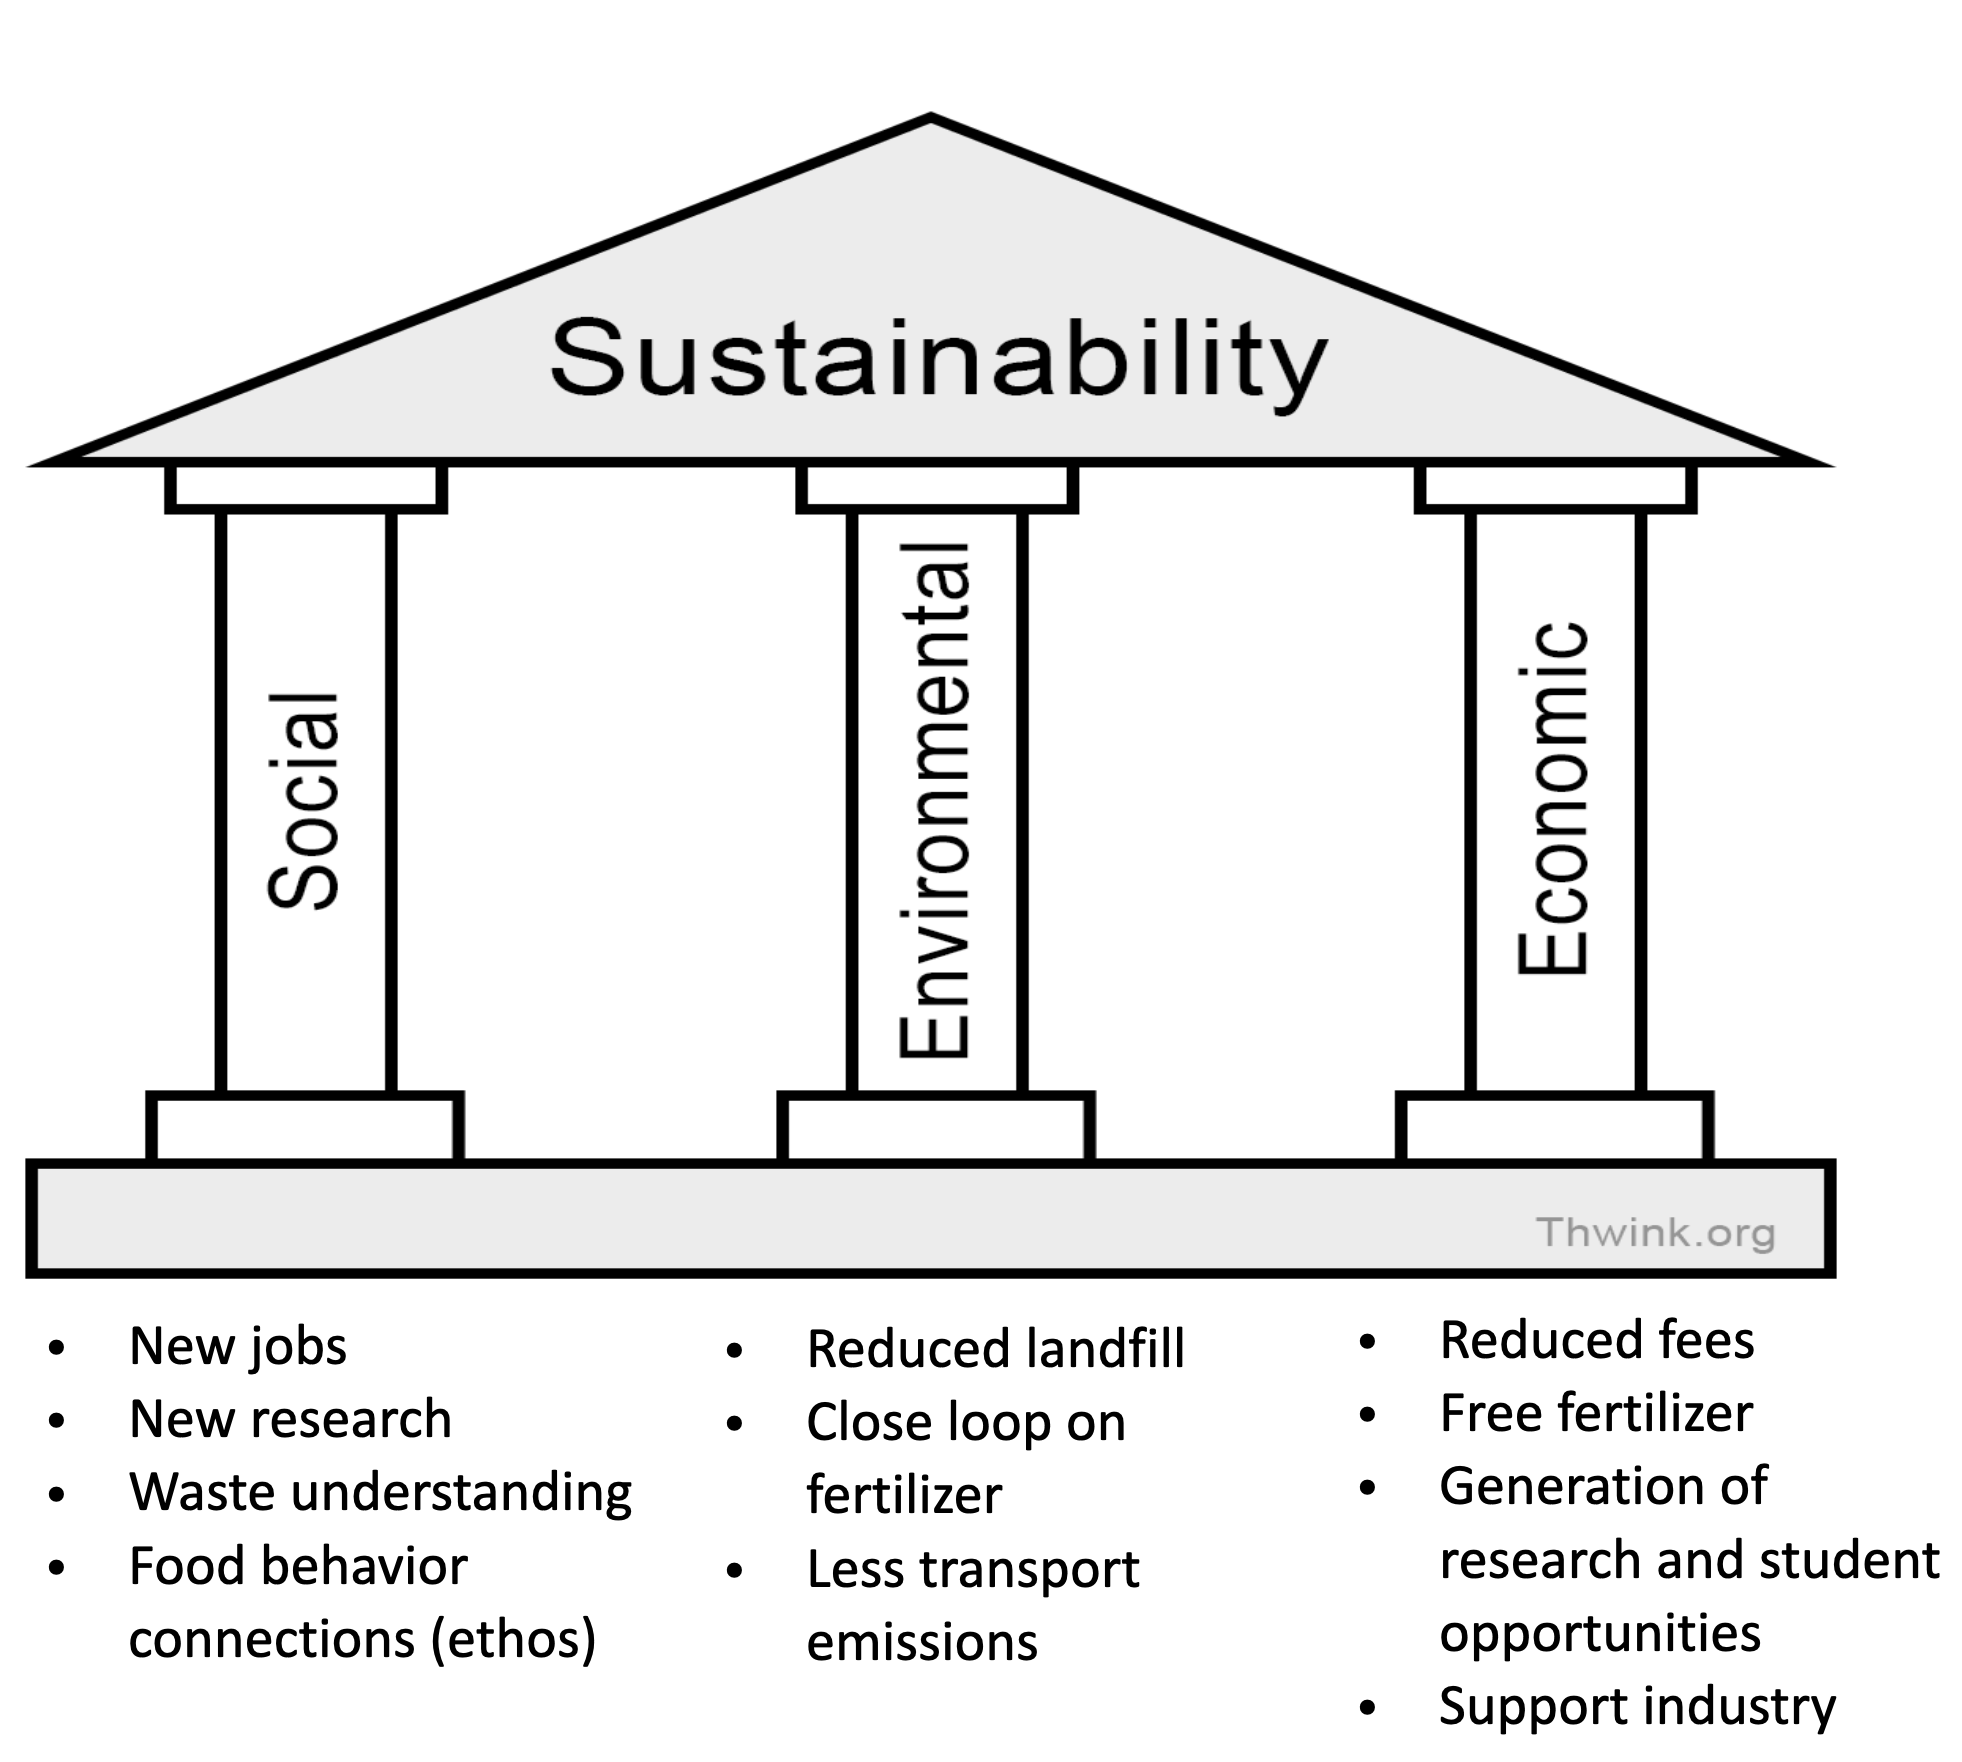
\includegraphics{asset/threepillars.png} - Three pillars of
sustainability - 17 SDGs - Logistics \& introduction to group project
\end{frame}

\begin{frame}{2: Overview for this week}
\phantomsection\label{overview-for-this-week}
\begin{itemize}
\tightlist
\item
  Refresh knowledge of SDGs and the three pillars of sustainability
\item
  Understand the triple bottom line concept
\item
  Explore key sustainability principles
\item
  Real-world examples of sustinable leadership principles
\end{itemize}
\end{frame}

\begin{frame}{3: Sustainable Development Goals (SDGs)}
\phantomsection\label{sustainable-development-goals-sdgs}
\begin{figure}[H]

{\centering 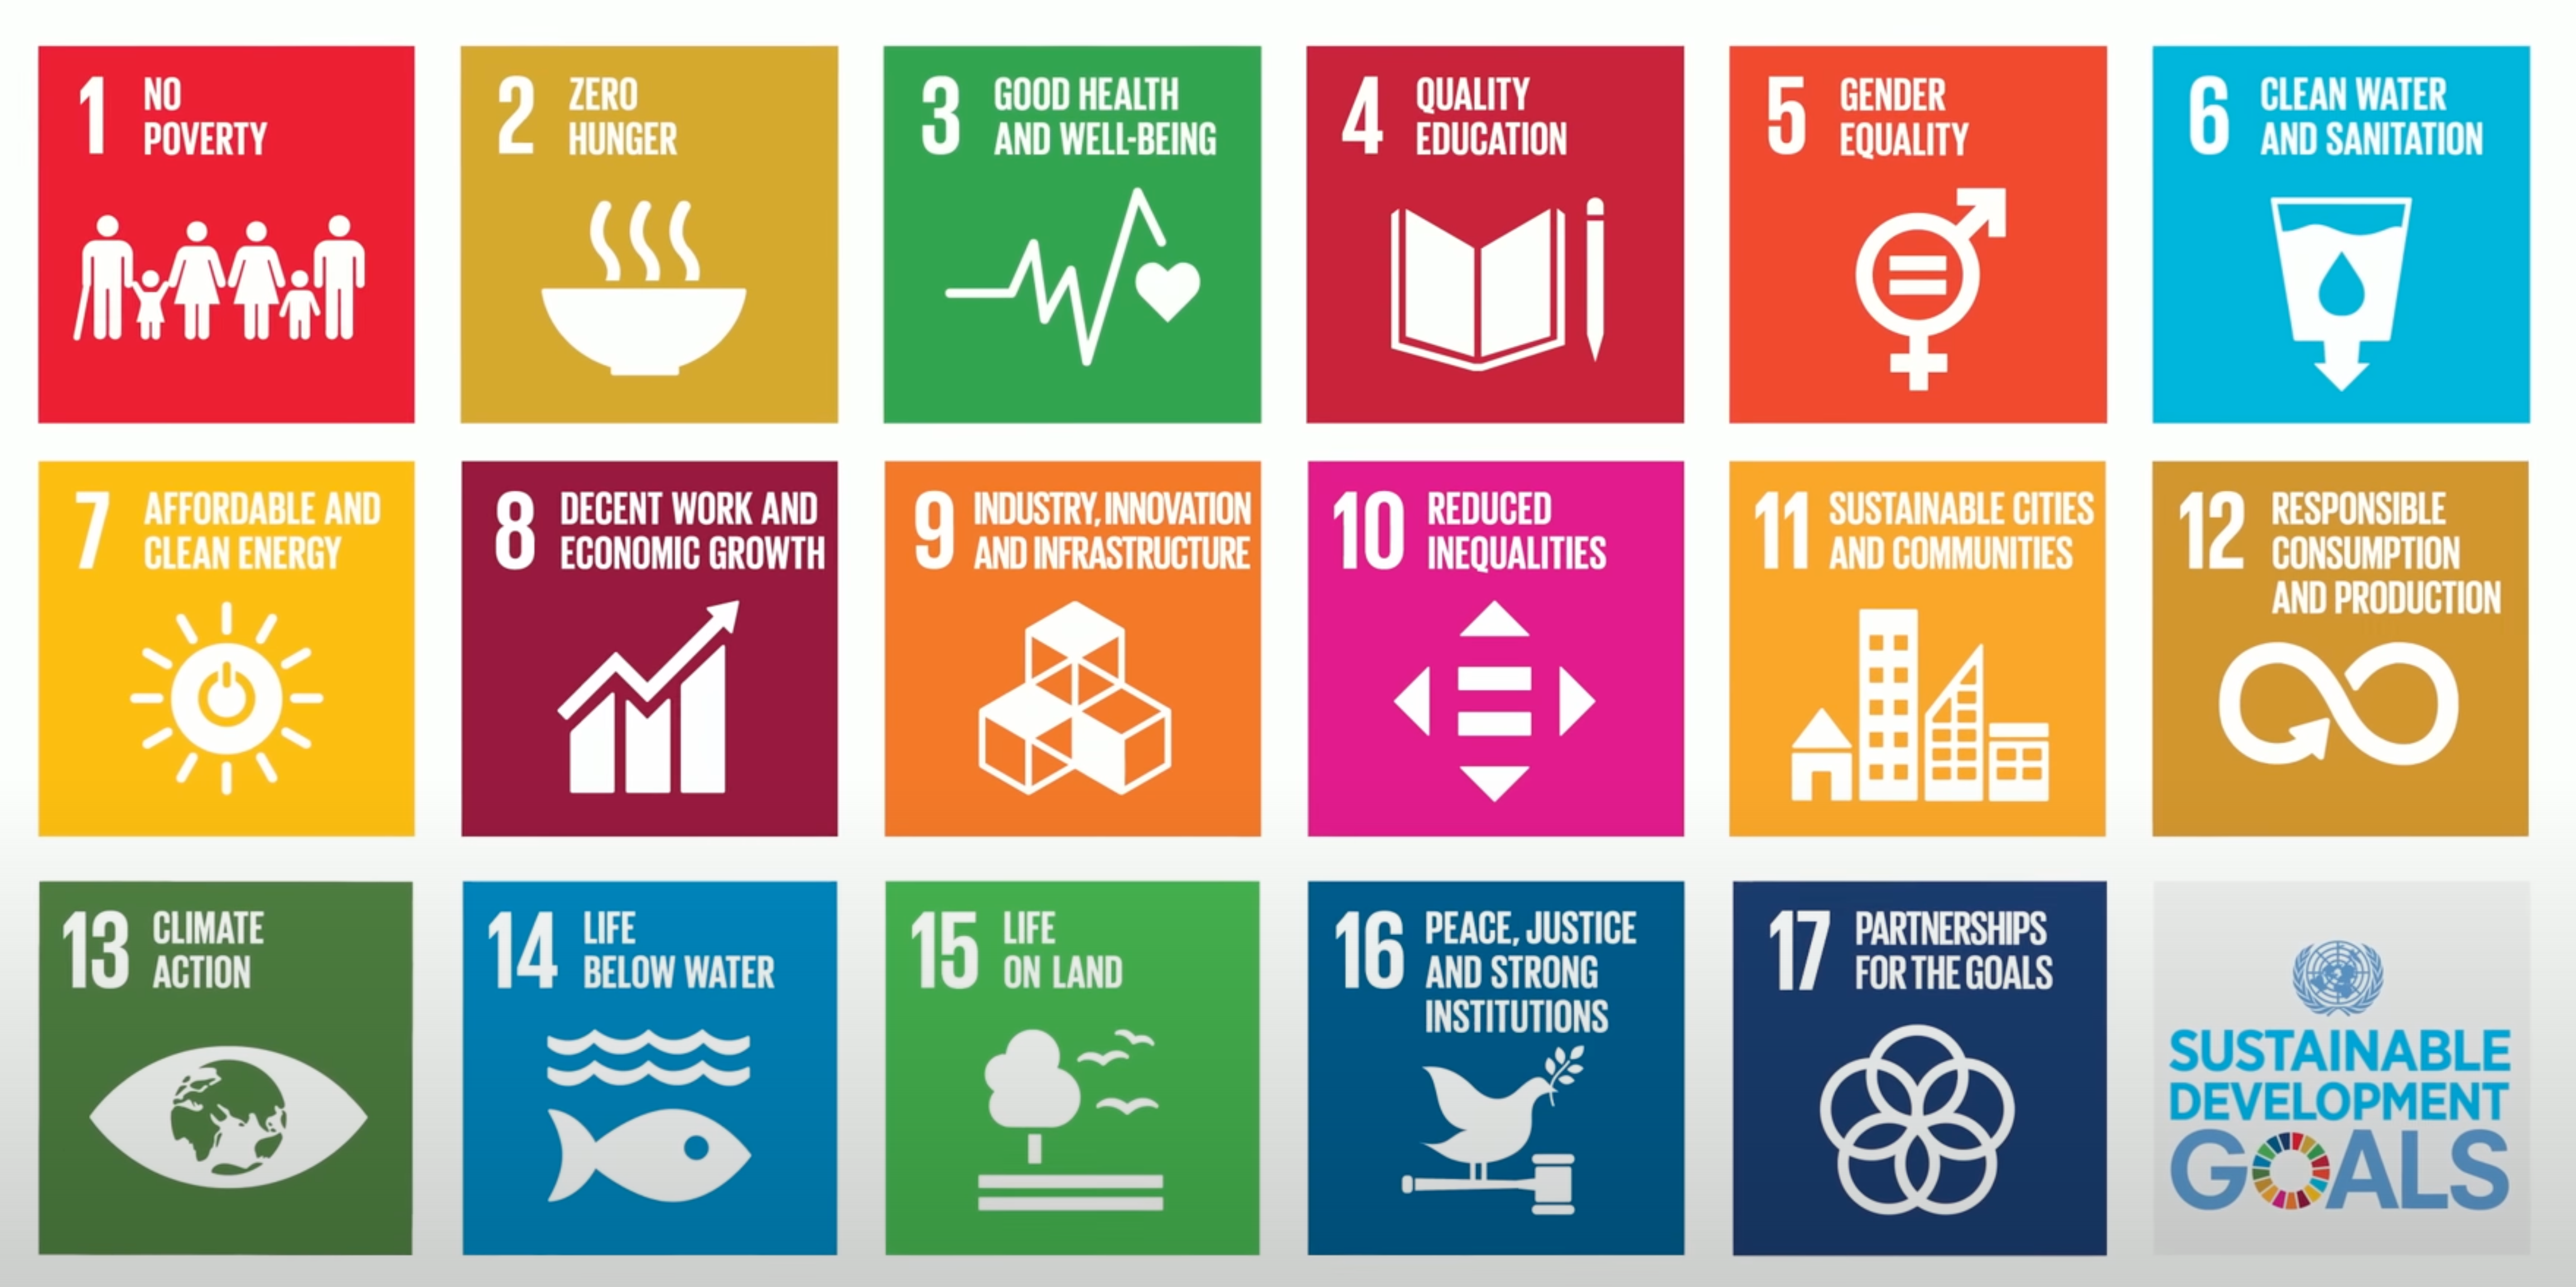
\includegraphics[width=0.7\textwidth,height=\textheight]{asset/SDGs17.png}

}

\caption{17 SDG Goals}

\end{figure}%

``United Nations Sustainable Development Goals, adopted in 2015''
\end{frame}

\begin{frame}{4: Three Pillars of Sustainability}
\phantomsection\label{three-pillars-of-sustainability}
\begin{itemize}
\tightlist
\item
  Title: ``The Three Pillars of Sustainability''
\item
  Venn Diagram: Venn diagram with three overlapping circles

  \begin{itemize}
  \tightlist
  \item
    Environmental Sustainability
  \item
    Social Sustainability
  \item
    Economic Sustainability
  \end{itemize}
\end{itemize}

\begin{figure}[H]

{\centering 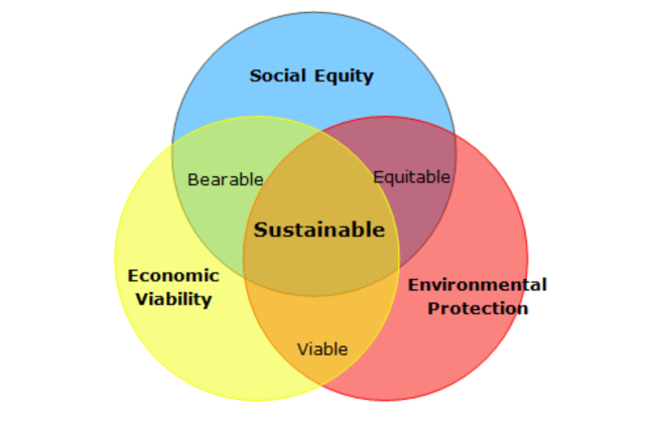
\includegraphics[width=0.4\textwidth,height=\textheight]{L2_files/mediabag/444c0baa-7e22-4182-9.png}

}

\caption{Venn Diagram of Sustainability}

\end{figure}%
\end{frame}

\begin{frame}{5: From Pillars to Triple Bottom Line}
\phantomsection\label{from-pillars-to-triple-bottom-line}
\begin{itemize}
\tightlist
\item
  Title: ``Evolving Concepts: Pillars to Triple Bottom Line''
\item
  Three Pillars → Triple Bottom Line

  \begin{itemize}
  \tightlist
  \item
    Social → People
  \item
    Environmental → Planet
  \item
    Economic → Profit
  \end{itemize}
\end{itemize}
\end{frame}

\begin{frame}[fragile]{6: The Triple Bottom Line}
\phantomsection\label{the-triple-bottom-line}
\begin{itemize}
\tightlist
\item
  Brief explanation of each component:

  \begin{itemize}
  \tightlist
  \item
    \texttt{People}: An organization's commitment to positively
    impacting society
  \item
    \texttt{Planet}: An organization's effect on the environment
  \item
    \texttt{Profit}: The financial return an orgnization generates for
    shareholders
  \end{itemize}
\item
  \textbf{Interconnectedness and balance}
\end{itemize}
\end{frame}

\begin{frame}{7: Patagonia's Triple Bottom Line Approach, a Case Study}
\phantomsection\label{patagonias-triple-bottom-line-approach-a-case-study}

\includegraphics[width=0.7\textwidth,height=\textheight]{asset/patagonia-logo-720.jpg}
\end{frame}

\begin{frame}{8: Patagonia's Triple Bottom Line Approach}
\phantomsection\label{patagonias-triple-bottom-line-approach}
\begin{enumerate}
\tightlist
\item
  People (Social)

  \begin{itemize}
  \tightlist
  \item
    Fair Labor Practices: Ensures fair wages and safe working conditions
  \item
    Activism: Supports environmental causes and encourages civic
    engagement
  \end{itemize}
\item
  Planet (Environmental)

  \begin{itemize}
  \tightlist
  \item
    Sustainable Materials: Uses recycled and organic materials
  \item
    Repair and Reuse: ``Worn Wear'' program to extend product life
  \end{itemize}
\item
  Profit (Economic)

  \begin{itemize}
  \tightlist
  \item
    Sustainable Business Model: Premium pricing for quality, durable
    products
  \item
    Long-term Growth: Brand loyalty through commitment to values
  \end{itemize}
\end{enumerate}

\textbf{Prioritizing people and planet can lead to long-term
profitability and brand strength.}
\end{frame}

\begin{frame}{7: Unilever Overview}
\phantomsection\label{unilever-overview}
\begin{itemize}
\tightlist
\item
  Multinational consumer goods company
\item
  Launched the Sustainable Living Plan in 2010
\item
  Goal: Double the business while halving environmental footprint
\end{itemize}
\end{frame}

\begin{frame}{8: Unilever's Triple Bottom Line Approach}
\phantomsection\label{unilevers-triple-bottom-line-approach}
\begin{enumerate}
\tightlist
\item
  People (Social)

  \begin{itemize}
  \tightlist
  \item
    Enhancing Livelihoods: Reached 2.34 million smallholder farmers
    through initiatives
  \item
    Improving Health and Well-being: Helped 1.3 billion people improve
    health and hygiene
  \end{itemize}
\item
  Planet (Environmental)

  \begin{itemize}
  \tightlist
  \item
    Sustainable Sourcing: 62\% of agricultural raw materials sustainably
    sourced
  \item
    Waste Reduction: Achieved zero non-hazardous waste to landfill
    across global factory network
  \end{itemize}
\item
  Profit (Economic)

  \begin{itemize}
  \tightlist
  \item
    Sustainable Living Brands: Grew 69\% faster than the rest of the
    business
  \item
    Cost Savings: €1 billion saved through eco-efficiency measures in
    factories since 2008
  \end{itemize}
\end{enumerate}
\end{frame}

\begin{frame}{9: Unilever's Impact}
\phantomsection\label{unilevers-impact}
\begin{itemize}
\tightlist
\item
  Key Achievements:

  \begin{itemize}
  \tightlist
  \item
    Reduced CO2 emissions by 52\% per tonne of production since 2008
  \item
    56\% of agricultural raw materials sustainably sourced
  \item
    1.85 million women enabled to access initiatives aiming to promote
    their safety
  \end{itemize}
\item
  Challenges:

  \begin{itemize}
  \tightlist
  \item
    Plastic packaging remains an issue
  \item
    Balancing growth with absolute reduction in environmental impact
  \end{itemize}
\end{itemize}
\end{frame}

\begin{frame}{10: Key Takeaways}
\phantomsection\label{key-takeaways}
\begin{itemize}
\tightlist
\item
  Successful implementation of triple bottom line requires long-term
  commitment
\item
  Integration of sustainability into core business strategy is crucial
\item
  Transparency and measurable goals are important for accountability
\item
  Challenges remain, particularly in achieving absolute reductions while
  growing business
\end{itemize}
\end{frame}

\section{Going further into
Principles}\label{going-further-into-principles}

\begin{frame}{11: Key Sustainability Principles}
\phantomsection\label{key-sustainability-principles}
\begin{itemize}
\tightlist
\item
  Precautionary Principle
\item
  Intergenerational Equity
\item
  \textbf{Systems Thinking}: Interconnected Everything
\item
  Circular Economy: \emph{Cradle-to-Cradle}
\item
  Stakeholder Engagement
\end{itemize}
\end{frame}

\begin{frame}{12: Systems Thinking}
\phantomsection\label{systems-thinking}
\begin{figure}[H]

{\centering \includegraphics[width=\textwidth,height=0.9\textheight]{L2_files/mediabag/thinking-in-systems-.png}

}

\caption{``Thinking in Systems : A Primer'' by Donella Meadows}

\end{figure}%
\end{frame}

\begin{frame}[fragile]{12.1: Systems Thinking in Sustainability}
\phantomsection\label{systems-thinking-in-sustainability}
\begin{itemize}
\tightlist
\item
  Definition: Considering the \texttt{interconnectedness} of various
  elements within a system
\item
  Key aspects:

  \begin{enumerate}
  \tightlist
  \item
    \textbf{Holistic} view
  \item
    Feedback \textbf{loops}
  \item
    Emergent properties
  \item
    Non-linear relationships
  \end{enumerate}
\end{itemize}
\end{frame}

\begin{frame}{13: Applying Sustainability Principles in Decision-Making}
\phantomsection\label{applying-sustainability-principles-in-decision-making}
\begin{itemize}
\tightlist
\item
  Framework:

  \begin{enumerate}
  \tightlist
  \item
    Identify the issue
  \item
    Apply relevant principles
  \item
    Consider stakeholders
  \item
    Assess short and long-term impacts
  \item
    Evaluate alternatives
  \item
    Implement and monitor
  \end{enumerate}
\end{itemize}
\end{frame}

\begin{frame}{14: Case Study - Wildlife Conservation and Ecosystem
Balance}
\phantomsection\label{case-study---wildlife-conservation-and-ecosystem-balance}
\begin{itemize}
\tightlist
\item
  Challenge: Balancing wildlife conservation with human needs in African
  savannas
\item
  Principles applied: Systems Thinking, Precautionary Principle,
  Stakeholder Engagement
\end{itemize}
\end{frame}

\begin{frame}{15: ``Return of the Wolves''}
\phantomsection\label{return-of-the-wolves}
When wolves were reintroduced to Yellowstone National Park in 1995, it
triggered a trophic cascade that changed the rivers. The wolves kept elk
populations in check, allowing trees to recover, which stabilized
riverbanks and changed the course of rivers. This showcases the
intricate connections in ecosystems.
\end{frame}

\begin{frame}{}
\phantomsection\label{section}
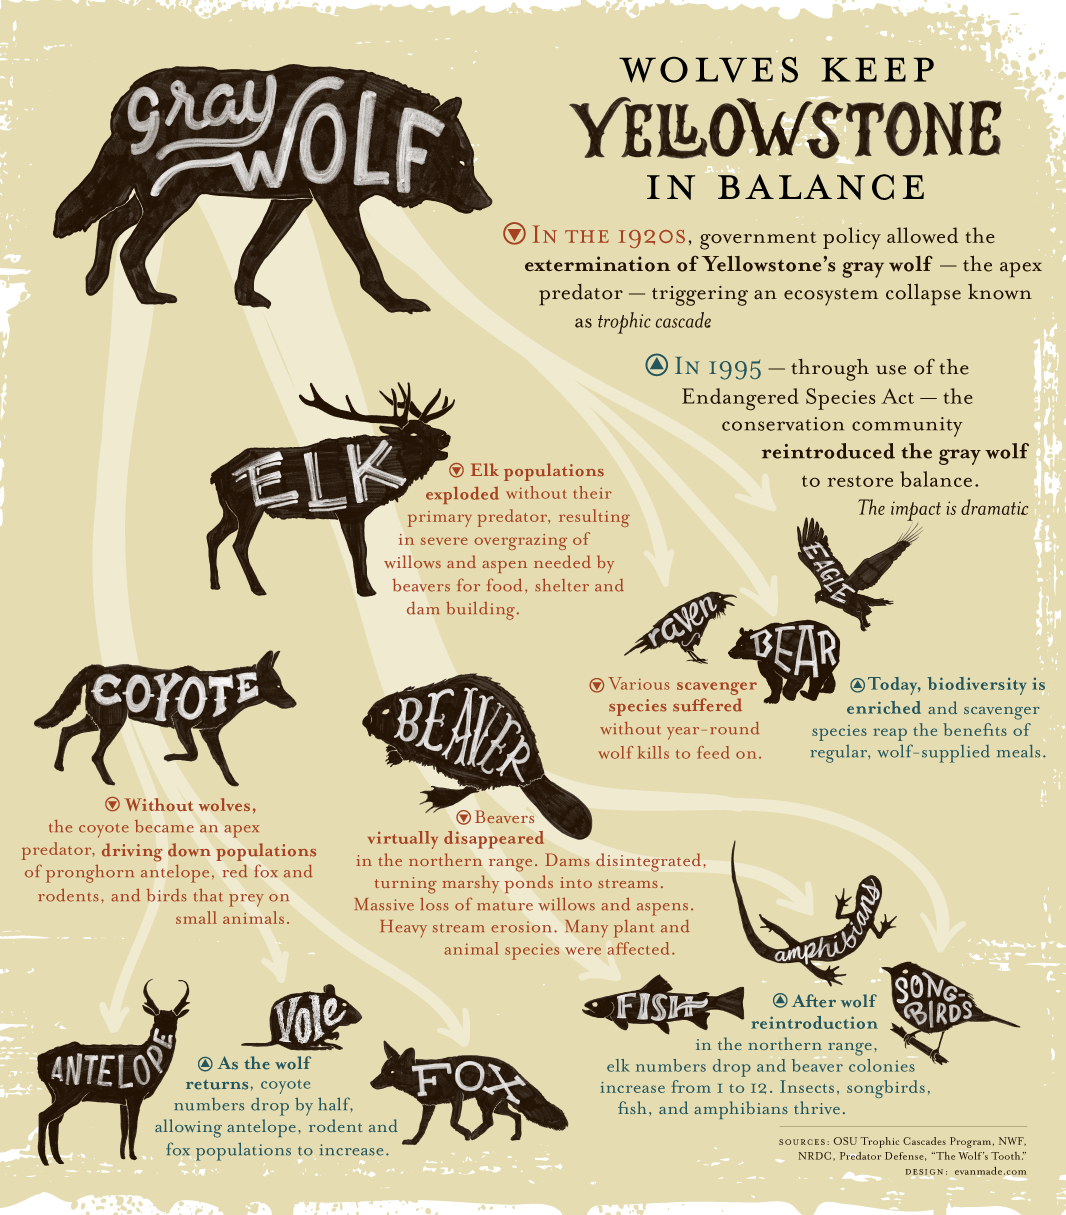
\includegraphics[width=\textwidth,height=0.8\textheight]{L2_files/mediabag/infographic-wolves_1.png}

EARTHJUSTICE, Infographic: Wolves Keep Yellowstone in the Balance,
February 2, 2015, Retrieved on Sep 8th, 2024 from
https://earthjustice.org/feature/infographic-wolves-keep-yellowstone-in-the-balance
\end{frame}

\section{Concluding Notes}\label{concluding-notes}

\begin{frame}{16: Recap of Key Concepts}
\phantomsection\label{recap-of-key-concepts}
\begin{itemize}
\tightlist
\item
  Sustainable Development Goals (SDGs)
\item
  Three Pillars of Sustainability

  \begin{itemize}
  \tightlist
  \item
    Environmental
  \item
    Social
  \item
    Economic
  \end{itemize}
\item
  Triple Bottom Line

  \begin{itemize}
  \tightlist
  \item
    People
  \item
    Planet
  \item
    Profit
  \end{itemize}
\item
  Key Sustainability Principles

  \begin{itemize}
  \tightlist
  \item
    Systems Thinking
  \item
    Precautionary Principle
  \item
    Intergenerational Equity
  \item
    Resource Efficiency
  \item
    Stakeholder Engagement
  \end{itemize}
\end{itemize}
\end{frame}

\begin{frame}{17: Applying Sustainability Principles in Practice}
\phantomsection\label{applying-sustainability-principles-in-practice}
\begin{itemize}
\tightlist
\item
  Systems Thinking as a Foundation

  \begin{itemize}
  \tightlist
  \item
    Understanding interconnections
  \item
    Recognizing feedback loops
  \item
    Anticipating unintended consequences
  \end{itemize}
\item
  Decision-Making Framework

  \begin{enumerate}
  \tightlist
  \item
    Define the problem holistically
  \item
    Engage stakeholders
  \item
    Apply relevant sustainability principles
  \item
    Assess short and long-term impacts
  \item
    Implement and monitor adaptively
  \end{enumerate}
\end{itemize}
\end{frame}

\begin{frame}{18: Additional Resources}
\phantomsection\label{additional-resources}
\begin{itemize}
\tightlist
\item
  \href{https://sdgs.un.org/goals}{UN Sustainable Development Goals}
\item
  \href{https://www.ellenmacarthurfoundation.org}{Ellen MacArthur
  Foundation} (Circular Economy)
\item
  \href{https://www.wbcsd.org}{World Business Council for Sustainable
  Development}
\item
  Recommended Reading:

  \begin{itemize}
  \tightlist
  \item
    ``Thinking in Systems'' by Donella Meadows
  \item
    ``Cradle to Cradle'' by William McDonough \& Michael Braungart
  \item
    ``The Limits to Growth'' by Donella Meadows, Dennis Meadows, Jørgen
    Randers
  \end{itemize}
\end{itemize}
\end{frame}

\section{Additional Cases just for
fun}\label{additional-cases-just-for-fun}

\begin{frame}{The Three Sisters}
\phantomsection\label{the-three-sisters}
\begin{itemize}
\tightlist
\item
  ``The Three Sisters'': Native American farming technique of planting
  corn, beans, and squash together. The corn provides a structure for
  the beans to climb, the beans fix nitrogen in the soil, and the squash
  spreads along the ground preventing weeds. It's a perfect example of
  \emph{companion planting and systems thinking in agriculture}.
\end{itemize}

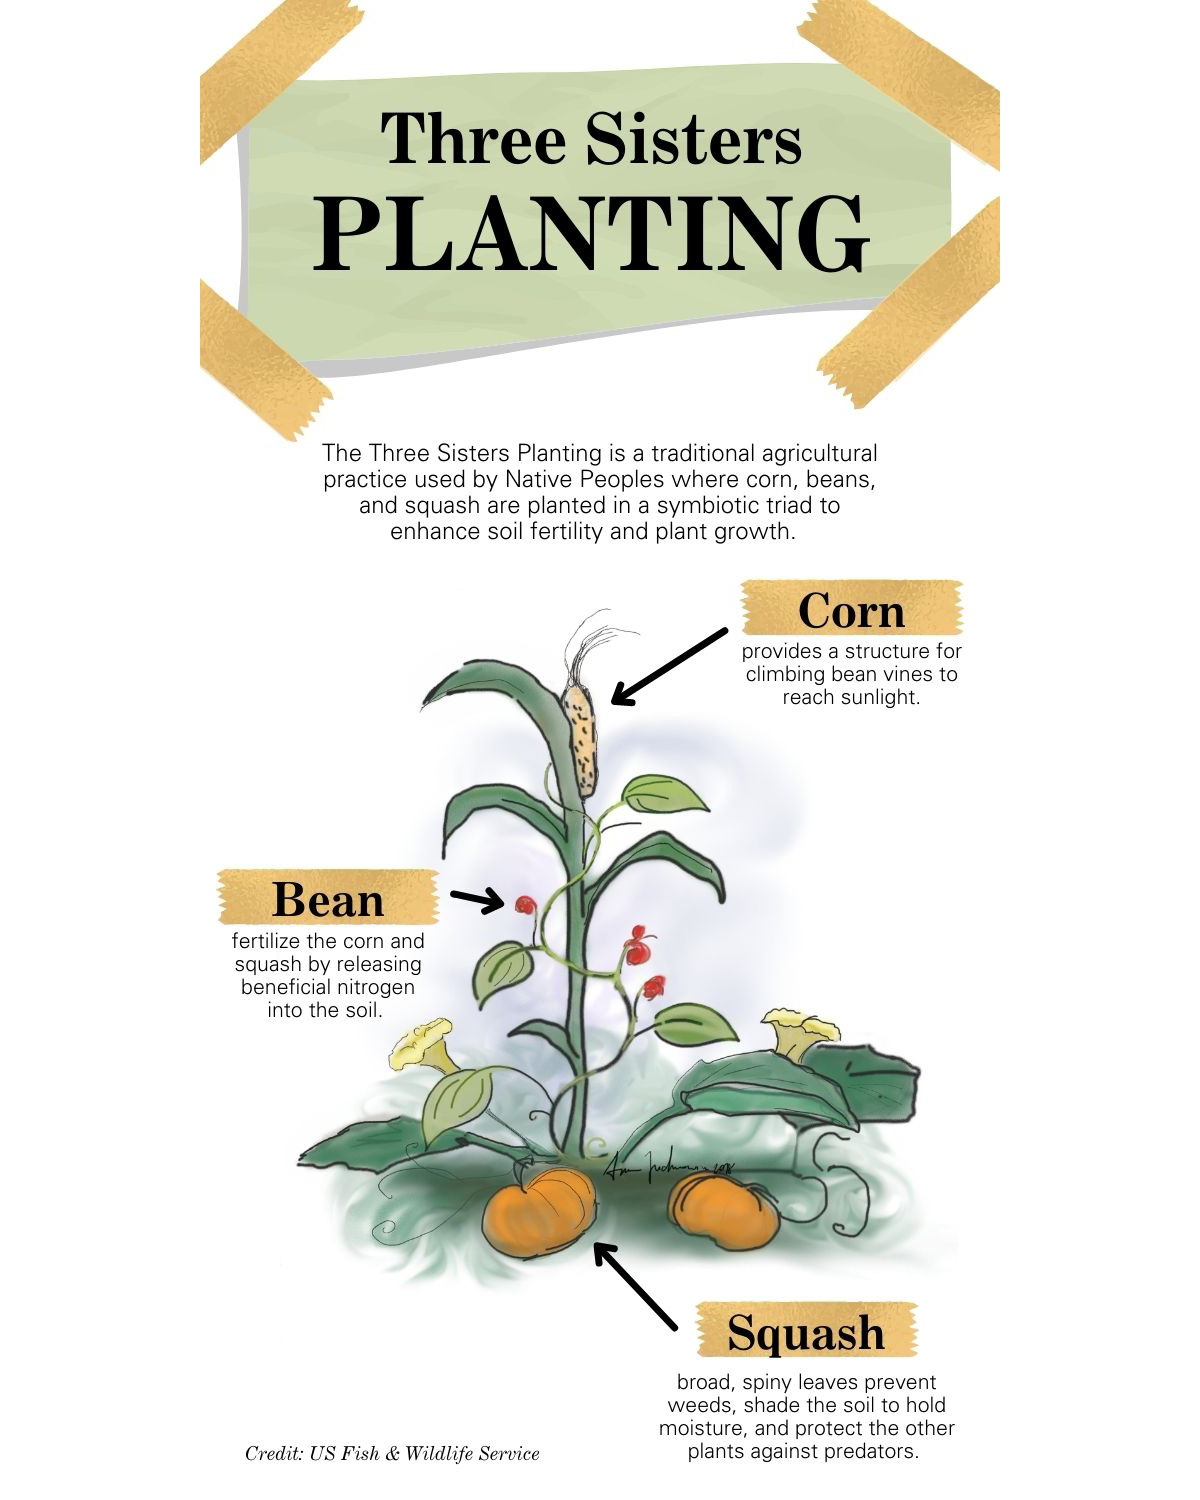
\includegraphics[width=0.3\textwidth,height=\textheight]{L2_files/mediabag/three-sisters-planti.jpg}
\end{frame}

\begin{frame}{The Duck Curve}
\phantomsection\label{the-duck-curve}
\begin{itemize}
\tightlist
\item
  ``The Duck Curve'': California's energy grid faces a unique challenge
  called the ``duck curve.'' As solar power increases during the day,
  traditional power plants need to rapidly ramp up production when the
  sun sets. The graph of this phenomenon looks like a duck, hence the
  name. It's a great example of the complexities in transitioning to
  renewable energy.
\end{itemize}

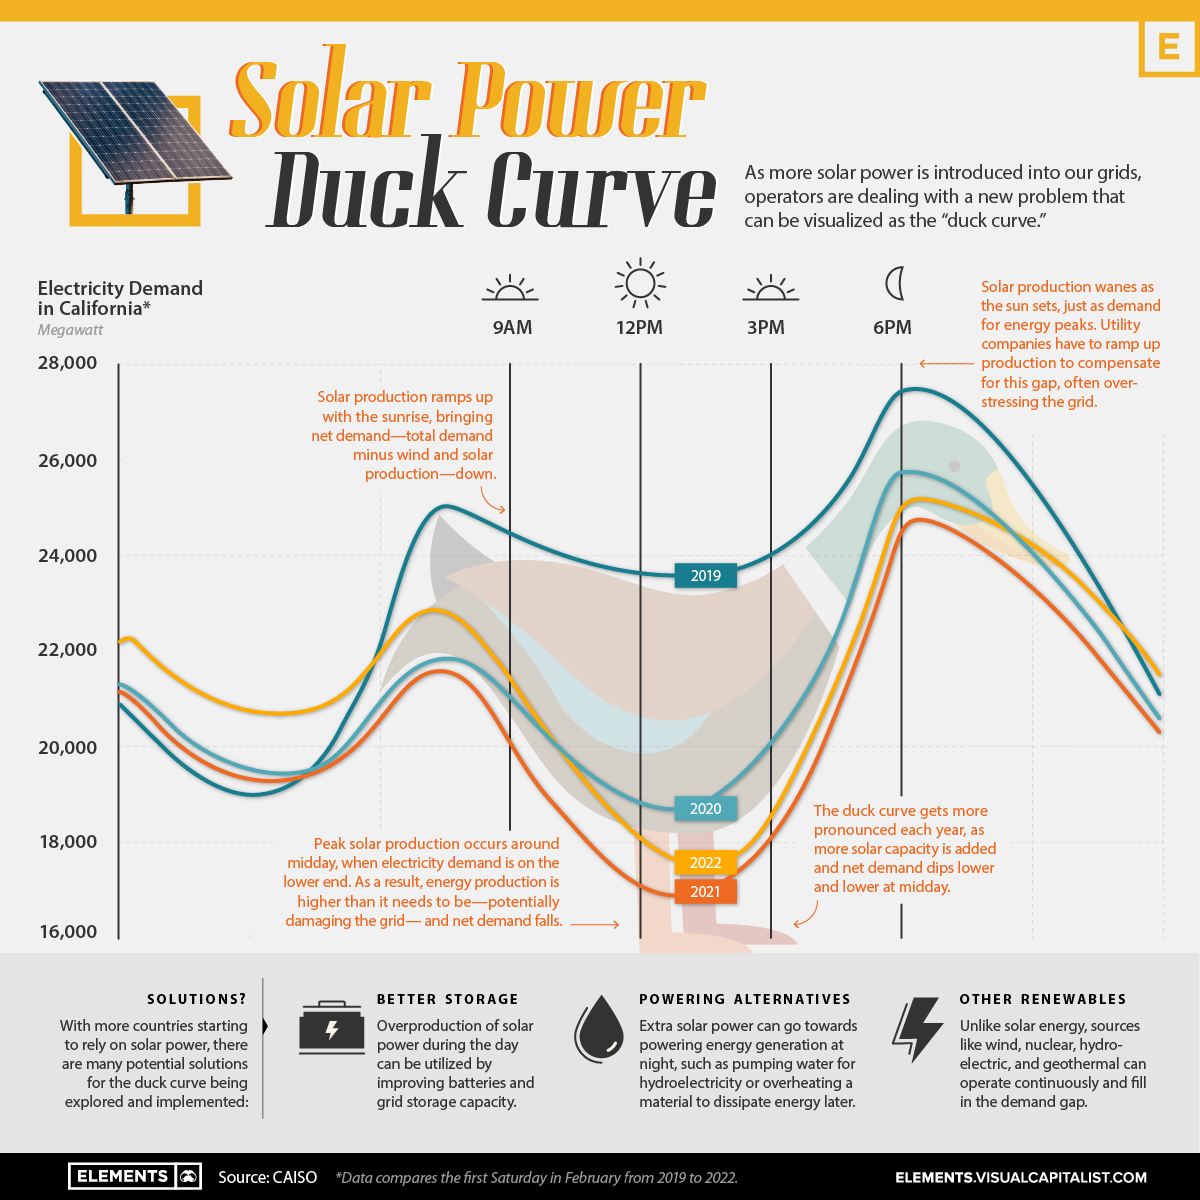
\includegraphics[width=0.5\textwidth,height=\textheight]{L2_files/mediabag/VCE-The-Duck-Curve-M.jpg}
\end{frame}

\begin{frame}{``The Great Horse Manure Crisis of 1894'':}
\phantomsection\label{the-great-horse-manure-crisis-of-1894}
In the late 19th century, large cities faced a growing problem with
horse manure from transportation. Some predicted London would be buried
under 9 feet of manure by 1950. This crisis was averted not by better
manure management, but by the invention of the automobile. It
demonstrates how technological innovations can solve sustainability
challenges in unexpected ways.

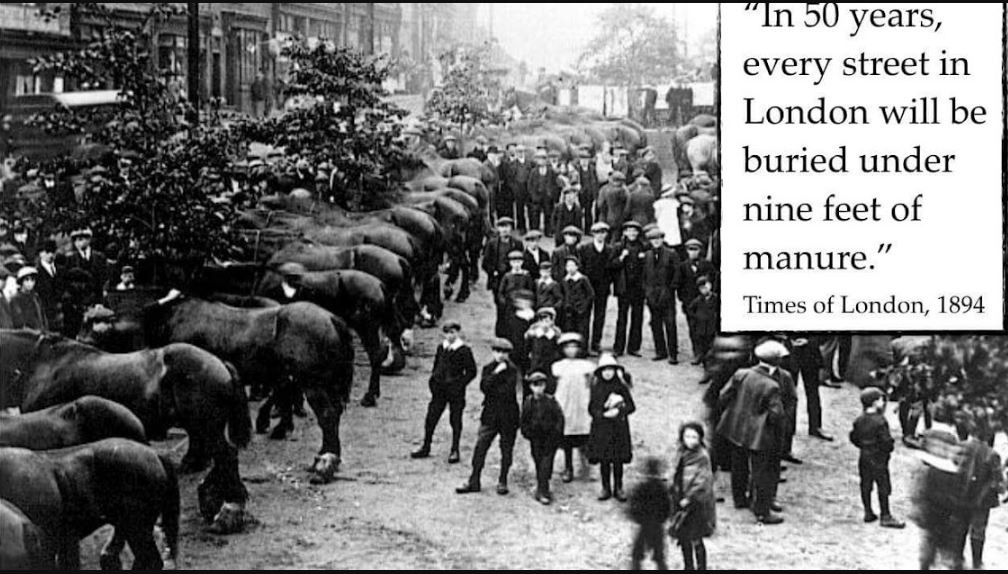
\includegraphics[width=0.5\textwidth,height=\textheight]{L2_files/mediabag/f22368cb-6608-4310-9.jpg}
\end{frame}



\end{document}
